\graphicspath{ {images/} }

\titledquestion{Analyzing NMT Systems}[25]

\begin{parts}

    \part[3] Look at the {\monofam{src.vocab}} file for some examples of phrases and words in the source language vocabulary. When encoding an input Mandarin Chinese sequence into ``pieces'' in the vocabulary, the tokenizer maps the sequence to a series of vocabulary items, each consisting of one or more characters (thanks to the {\monofam{sentencepiece}} tokenizer, we can perform this segmentation even when the original text has no white space). Given this information, how could adding a 1D Convolutional layer after the embedding layer and before passing the embeddings into the bidirectional encoder help our NMT system? \textbf{Hint:} each Mandarin Chinese character is either an entire word or a morpheme in a word. Look up the meanings of 电, 脑, and 电脑 separately for an example. The characters 电 (electricity) and  脑 (brain) when combined into the phrase 电脑 mean computer.


        \textcolor{red}{\textbf{Solution: } Adding a 1D Convolutional layer after the embedding layer can help the NMT system capture local patterns and relationships between characters in the Mandarin Chinese text. Since each character can represent a morpheme or an entire word, the convolutional layer can learn to recognize these patterns and relationships, allowing the model to better understand the meaning of phrases and words. This can lead to improved translation quality, as the model can better capture the semantics of the source language. Additionally, the convolutional layer can help reduce noise in the input by focusing on local features, which can further improve translation accuracy.}


    \part[8] Here we present a series of errors we found in the outputs of our NMT model (which is the same as the one you just trained). For each example of a reference (i.e., `gold') English translation, and NMT (i.e., `model') English translation, please:
    
    \begin{enumerate}
        \item Identify the error in the NMT translation.
        \item Provide possible reason(s) why the model may have made the error (either due to a specific linguistic construct or a specific model limitation).
        \item Describe one possible way we might alter the NMT system to fix the observed error. There are more than one possible fixes for an error. For example, it could be tweaking the size of the hidden layers or changing the attention mechanism.
    \end{enumerate}
    
    Below are the translations that you should analyze as described above. Only analyze the underlined error in each sentence. Rest assured that you don't need to know Mandarin to answer these questions. You just need to know English! If, however, you would like some additional color on the source sentences, feel free to use a resource like \url{https://www.archchinese.com/chinese_english_dictionary.html} to look up words. Feel free to search the training data file to have a better sense of how often certain characters occur.

    \begin{subparts}
        \subpart[2]
        \textbf{Source Sentence:} 贼人其后被警方拘捕及被判处盗窃罪名成立。 \newline
        \textbf{Reference Translation:} \textit{\underline{the culprits were} subsequently arrested and convicted.}\newline
        \textbf{NMT Translation:} \textit{\underline{the culprit was} subsequently arrested and sentenced to theft.}

        \textcolor{red}{\textbf{Solution: } The NMT translation incorrectly uses the singular form "culprit" instead of the plural "culprits". This could be due to the model's inability to correctly identify the plurality of the subject in the source sentence. To fix this, we could increase the size of the training data to include more examples of plural subjects, or we could implement a rule-based post-processing step that checks for subject-verb agreement.}
        

        \subpart[2]
        \textbf{Source Sentence}: 几乎已经没有地方容纳这些人,资源已经用尽。\newline
        \textbf{Reference Translation}: \textit{there is almost no space to accommodate these people, and resources have run out.   }\newline
        \textbf{NMT Translation}: \textit{the resources have been exhausted and \underline{resources have been exhausted}.}
        
        \textcolor{red}{\textbf{Solution: } The NMT translation repeats the phrase "resources have been exhausted" instead of translating the second part of the sentence. This could be due to a limitation in the model's ability to handle complex sentence structures or a lack of training data for similar sentences. To fix this, we could implement a more sophisticated attention mechanism that better captures the relationships between different parts of the sentence, or we could increase the size of the training data to include more examples of complex sentences.}
        

        \subpart[2]
        \textbf{Source Sentence}: 当局已经宣布今天是国殇日。 \newline
        \textbf{Reference Translation}: \textit{authorities have announced \underline{a national mourning today.}}\newline
        \textbf{NMT Translation}: \textit{the administration has announced \underline{today's day.}}
        
        \textcolor{red}{\textbf{Solution: } The NMT translation incorrectly translates "国殇日" as "today's day" instead of "a national mourning today". This could be due to the model's inability to recognize the specific term "国殇日" as a fixed expression. To fix this, we could implement a dictionary-based approach that maps specific terms to their correct translations, or we could increase the size of the training data to include more examples of fixed expressions.}
        
        
        \subpart[2] 
        \textbf{Source Sentence\footnote{This is a Cantonese sentence! The data used in this assignment comes from GALE Phase 3, which is a compilation of news written in simplified Chinese from various sources scraped from the internet along with their translations. For more details, see \url{https://catalog.ldc.upenn.edu/LDC2017T02}. }:} 俗语有云:``唔做唔错"。\newline
        \textbf{Reference Translation:} \textit{\underline{`` act not, err not "}, so a saying goes.}\newline
        \textbf{NMT Translation:} \textit{as the saying goes, \underline{`` it's not wrong. "}}

        \textcolor{red}{\textbf{Solution: } The NMT translation incorrectly translates the Cantonese phrase "唔做唔错" as "it's not wrong" instead of " act not, err not ". This could be due to the model's inability to handle idiomatic expressions or fixed phrases in Cantonese. To fix this, we could implement a rule-based post-processing step that identifies and correctly translates idiomatic expressions, or we could increase the size of the training data to include more examples of idiomatic expressions in Cantonese.}
        
        
    \end{subparts}


    \part[14] BLEU score is the most commonly used automatic evaluation metric for NMT systems. It is usually calculated across the entire test set, but here we will consider BLEU defined for a single example.\footnote{This definition of sentence-level BLEU score matches the \texttt{sentence\_bleu()} function in the \texttt{nltk} Python package. Note that the NLTK function is sensitive to capitalization. In this question, all text is lowercased, so capitalization is irrelevant. \\ \url{http://www.nltk.org/api/nltk.translate.html\#nltk.translate.bleu_score.sentence_bleu}
    } 
    Suppose we have a source sentence $\bs$, a set of $k$ reference translations $\br_1,\dots,\br_k$, and a candidate translation $\bc$. To compute the BLEU score of $\bc$, we first compute the \textit{modified $n$-gram precision} $p_n$ of $\bc$, for each of $n=1,2,3,4$, where $n$ is the $n$ in \href{https://en.wikipedia.org/wiki/N-gram}{n-gram}:
    \begin{align}
        p_n = \frac{ \displaystyle \sum_{\text{ngram} \in \bc} \min \bigg( \max_{i=1,\dots,k} \text{Count}_{\br_i}(\text{ngram}), \enspace \text{Count}_{\bc}(\text{ngram}) \bigg) }{\displaystyle \sum_{\text{ngram}\in \bc} \text{Count}_{\bc}(\text{ngram})}
    \end{align}
     Here, for each of the $n$-grams that appear in the candidate translation $\bc$, we count the maximum number of times it appears in any one reference translation, capped by the number of times it appears in $\bc$ (this is the numerator). We divide this by the number of $n$-grams in $\bc$ (denominator). \newline 

    Next, we compute the \textit{brevity penalty} BP. Let $len(c)$ be the length of $\bc$ and let $len(r)$ be the length of the reference translation that is closest to $len(c)$ (in the case of two equally-close reference translation lengths, choose $len(r)$ as the shorter one). 
    \begin{align}
        BP = 
        \begin{cases}
            1 & \text{if } len(c) \ge len(r) \\
            \exp \big( 1 - \frac{len(r)}{len(c)} \big) & \text{otherwise}
        \end{cases}
    \end{align}
    Lastly, the BLEU score for candidate $\bc$ with respect to $\br_1,\dots,\br_k$ is:
    \begin{align}
        BLEU = BP \times \exp \Big( \sum_{n=1}^4 \lambda_n \log p_n \Big)
    \end{align}
    where $\lambda_1,\lambda_2,\lambda_3,\lambda_4$ are weights that sum to 1. The $\log$ here is natural log.
    \newline
    \begin{subparts}
        \subpart[5] Please consider this example: \newline
        Source Sentence $\bs$: \textbf{需要有充足和可预测的资源。} 
        \newline
        Reference Translation $\br_1$: \textit{resources have to be sufficient and they have to be predictable}
        \newline
        Reference Translation $\br_2$: \textit{adequate and predictable resources are required}
        
        NMT Translation $\bc_1$: there is a need for adequate and predictable resources
        
        NMT Translation $\bc_2$: resources be sufficient and predictable to
        
        Please compute the BLEU scores for $\bc_1$ and $\bc_2$. Let $\lambda_i=0.5$ for $i\in\{1,2\}$ and $\lambda_i=0$ for $i\in\{3,4\}$ (\textbf{this means we ignore 3-grams and 4-grams}, i.e., don't compute $p_3$ or $p_4$). When computing BLEU scores, show your work (i.e., show your computed values for $p_1$, $p_2$, $len(c)$, $len(r)$ and $BP$). Note that the BLEU scores can be expressed between 0 and 1 or between 0 and 100. The code is using the 0 to 100 scale while in this question we are using the \textbf{0 to 1} scale. Please round your responses to 3 decimal places. 

        \ifans{
            \newline
            For $\bc_1$:

            \begin{align*}
            p_1 &= \frac{0 + 0 + 0 + 0 + 0 + 1 + 1 + 1 + 1}{9} = \frac{4}{9} \approx 0.444 \\
            p_2 &= \frac{0 + 0 + 0 + 0 + 0 + 1 + 1 + 1}{8} = \frac{3}{8} \approx 0.375 \\
            len(c) &= 9 \\
            len(r) &= 11 \\
            BP &= \exp(1-\frac{11}{9}) \\
            BLEU &= BP \times \exp\Big(0.5\log(0.444) + 0.5\log(0.375)\Big) \approx 0.327 \\
            \end{align*}

            For $\bc_2$:
            \begin{align*}
            p_1 &= \frac{1 + 1 + 1 + 1 + 1 + 1}{6} = \frac{6}{6} = 1 \\
            p_2 &= \frac{0 + 1 + 1 + 1 + 0}{5} = \frac{3}{5} \approx 0.6 \\
            len(c) &= 6 \\
            len(r) &= 6 \\
            BP &= 1 \\
            BLEU &= BP \times \exp\Big(0.5\log(1) + 0.5\log(0.6)\Big) \approx 0.775
            \end{align*}
        }
        
        Which of the two NMT translations is considered the better translation according to the BLEU Score? Do you agree that it is the better translation?
        
        \ifans{
            \newline
            $\bc_2$ is considered the better translation according to the BLEU Score. However, I think that $bc_1$ is the better translation, as it is more fluent and captures the meaning of the source sentence better.
        }
        
        \subpart[5] Our hard drive was corrupted and we lost Reference Translation $\br_1$. Please recompute BLEU scores for $\bc_1$ and $\bc_2$, this time with respect to $\br_2$ only. Which of the two NMT translations now receives the higher BLEU score? Do you agree that it is the better translation?
        \ifans{
            \newline
            For $\bc_1$:

            \begin{align*}
            p_1 &= \frac{0 + 0 + 0 + 0 + 0 + 1 + 1 + 1 + 1}{9} = \frac{4}{9} \\
            p_2 &= \frac{0 + 0 + 0 + 0 + 0 + 1 + 1 + 1}{8} = \frac{3}{8} \\
            len(c) &= 9 \\
            len(r) &= 6 \\
            BP &= \exp(1-\frac{11}{9}) \\
            BLEU &= 1 \times \exp(0.5 \times \log{\frac{4}{9}} + 0.5 \times \log{\frac{3}{8}}) \approx 0.408
            \end{align*}

            For $\bc_2$:
            \begin{align*}
            p_1 &= \frac{1 + 0 + 0 + 1 + 1 + 0}{6} = \frac{3}{6} \\
            p_2 &= \frac{0 + 0 + 0 + 1 + 0}{5} = \frac{1}{5} \\
            len(c) &= 6 \\
            len(r) &= 6 \\
            BP &= 1 \\
            BLEU &= 1 \times \exp(0.5 \times \log{\frac{3}{6}} + 0.5 \times \log{\frac{1}{5}}) \approx 0.316
            \end{align*}

            Now, $\bc_1$ is considered the better translation according to the BLEU Score, which is reasonalbe as it is more fluent and captures the meaning of the source sentence better.
        }
        
        
        
        \subpart[2] Due to data availability, NMT systems are often evaluated with respect to only a single reference translation. Please explain (in a few sentences) why this may be problematic. In your explanation, discuss how the BLEU score metric assesses the quality of NMT translations when there are multiple reference transitions versus a single reference translation.

        \ifans{
            \newline
            Evaluating NMT systems with respect to only a single reference translation can be problematic because it does not capture the full range of possible translations for a given source sentence. Different reference translations may express the same meaning in different ways, and a single reference translation may not account for all of these variations. When there are multiple reference translations, the BLEU score metric assesses the quality of NMT translations by comparing them to all available references, allowing for a more comprehensive evaluation. In contrast, when there is only a single reference translation, the BLEU score may not accurately reflect the quality of the NMT translation, as it may not capture the full range of possible translations.
        }
        
        \subpart[2] List two advantages and two disadvantages of BLEU, compared to human evaluation, as an evaluation metric for Machine Translation. 
        
        \ifans{
            \newline
            Advantages:
            \begin{enumerate}
                \item BLEU is an automatic evaluation metric, which means it can be computed quickly and easily without the need for human annotators.
                \item BLEU is a widely used metric in the NMT community, which means it allows for easy comparison of different NMT systems and models.
            \end{enumerate}
            
            Disadvantages:
            \begin{enumerate}
                \item BLEU does not capture the full range of possible translations for a given source sentence, as it relies on a limited number of reference translations.
                \item BLEU does not account for the fluency or naturalness of the translation, as it only considers n-gram overlap between the candidate translation and reference translations.
            \end{enumerate}
        }
        
    \end{subparts}


    \part[4] \emph{Beam search} is often employed to improve the quality of machine translation systems. While you were training the model, beam search results for the same example sentence at different iterations were also recorded in TensorBoard, and accessible in the \emph{TEXT} tab (Fig \ref{fig:beam-search-diagnostics-tensorboard}).

    The recorded diagnostic information includes json documents with the following fields: \texttt{example\_source} (the source sentence tokens), \texttt{example\_target} (the ground truth target sentence tokens), and \texttt{hypotheses} (10 hypotheses corresponding to the search result with beam size 10). Note that a predicted translation is often called \emph{hypothesis} in the neural machine translation jargon.

    \begin{subparts}
        \subpart[2] Did the translation quality improve over the training iterations for the model? Give three examples of translations of the example sentence at iterations 200, 3000, and the last iteration to illustrate your answer. For each iteration, pick the first beam search hypothesis as an example:
        
        \ifans{
            \newline
            Yes, the translation quality improved over the training iterations.
            \begin{itemize}
                \item Iteration 800: \textit{I also also noted that the government had been a result of the united nations.}
                \item Iteration 4200: \textit{I have also clarified a number of matters raised by the meeting.}
                \item Last Iteration: \textit{I have also clarified a number of matters raised at the meeting.}
            \end{itemize}
        }
        
        
        \subpart[2] How do various hypotheses resulting from beam search qualitatively compare? Give three other examples of hypotheses proposed by beam search at the last iteration to illustrate your answer.
        
        \ifans{
            \newline
            The hypotheses resulting from beam search qualitatively compare in terms of fluency and accuracy. Some hypotheses are more fluent and natural-sounding, while others may be more literal translations.
            \begin{itemize}
                \item Hypothesis 1: \textit{I have also clarified a number of matters raised at the meeting.}
                \item Hypothesis 2: \textit{Clarification was also given to a number of matters raised at the meeting.}
                \item Hypothesis 3: \textit{I have also clarified a number of matters raised during the meeting".}
            \end{itemize}
        }
        
    \end{subparts}



    \begin{figure}
        \centering
        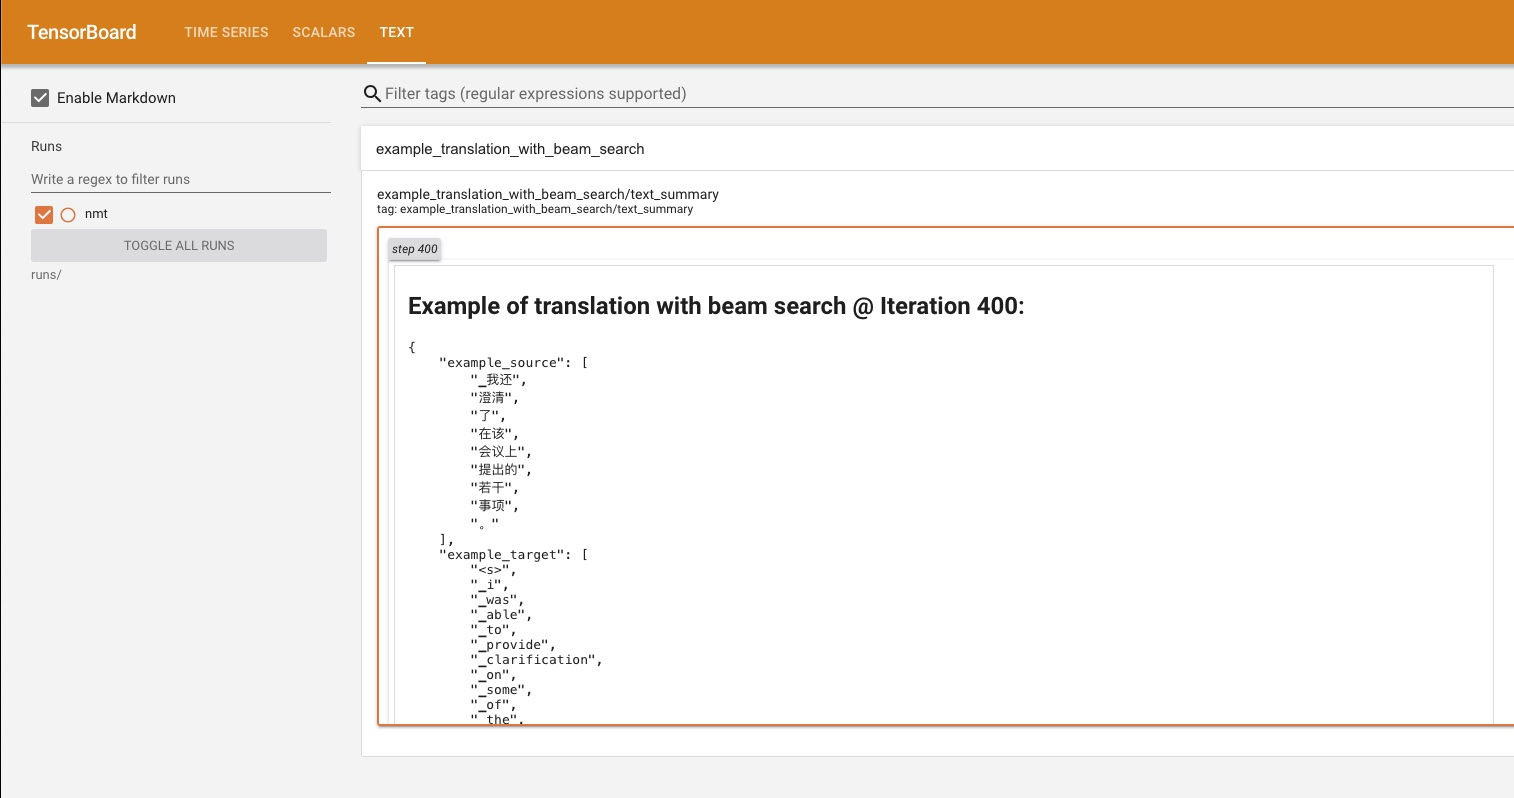
\includegraphics[width=0.7\textwidth]{images/example_translation_beam.jpg}
        \caption{Translation with beam search results for an example sentence are recorded in tensorboard for various iterations. The same data is available in the \texttt{outputs/beam\_search\_diagnostics/} folder in your working directory.}
        \label{fig:beam-search-diagnostics-tensorboard}
    \end{figure}
    

\end{parts}
